\documentclass[tikz,border=10pt]{standalone}
\usepackage{tikz}
\usetikzlibrary{positioning,arrows.meta,shapes,calc}

\begin{document}
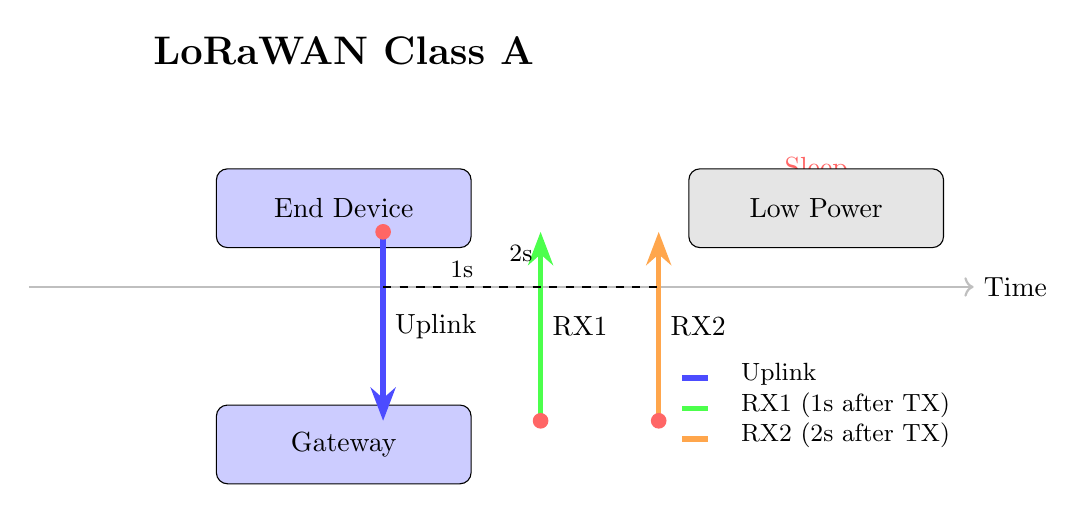
\begin{tikzpicture}[
    node distance=1.5cm,
    block/.style={rectangle, draw, fill=blue!20, text width=3cm, text centered, rounded corners, minimum height=1cm},
    arrow/.style={-Stealth, thick},
    timeline/.style={->, thick, draw=gray!50},
    event/.style={circle, fill=red!60, inner sep=2pt}
]

% Title
\node[font=\Large\bfseries] at (0,5) {LoRaWAN Class A};

% Device
\node[block] (device) at (0,3) {End Device};

% Gateway
\node[block] (gateway) at (0,0) {Gateway};

% Timeline
\draw[timeline] (-4,2) -- (8,2) node[right] {Time};

% Uplink
\draw[arrow, blue!70, line width=2pt] (0.5,2.7) -- node[right, black] {Uplink} (0.5,0.3);
\node[event] at (0.5,2.7) {};

% RX1 Window
\draw[arrow, green!70, line width=2pt] (2.5,0.3) -- node[right, black] {RX1} (2.5,2.7);
\node[event] at (2.5,0.3) {};
\draw[dashed] (0.5,2) -- (2.5,2);
\node[above] at (1.5,2) {\small 1s};

% RX2 Window
\draw[arrow, orange!70, line width=2pt] (4,0.3) -- node[right, black] {RX2} (4,2.7);
\node[event] at (4,0.3) {};
\draw[dashed] (0.5,2) -- (4,2);
\node[above] at (2.25,2.2) {\small 2s};

% Sleep period
\draw[<->, thick, red!60] (4.5,3.2) -- (7.5,3.2) node[midway, above] {Sleep};
\node[block, fill=gray!20] at (6,3) {Low Power};

% Legend
\node[font=\small] at (6,0.5) {
    \begin{tabular}{ll}
    \textcolor{blue!70}{\rule{1em}{2pt}} & Uplink \\
    \textcolor{green!70}{\rule{1em}{2pt}} & RX1 (1s after TX) \\
    \textcolor{orange!70}{\rule{1em}{2pt}} & RX2 (2s after TX) \\
    \end{tabular}
};

\end{tikzpicture}
\end{document}
